\documentclass[12pt]{article}
\usepackage{graphicx}

\pagestyle{empty}

\begin{document}

\subsection*{Layer 1 (Negative Z)}
  \begin{tabular}{c c}
    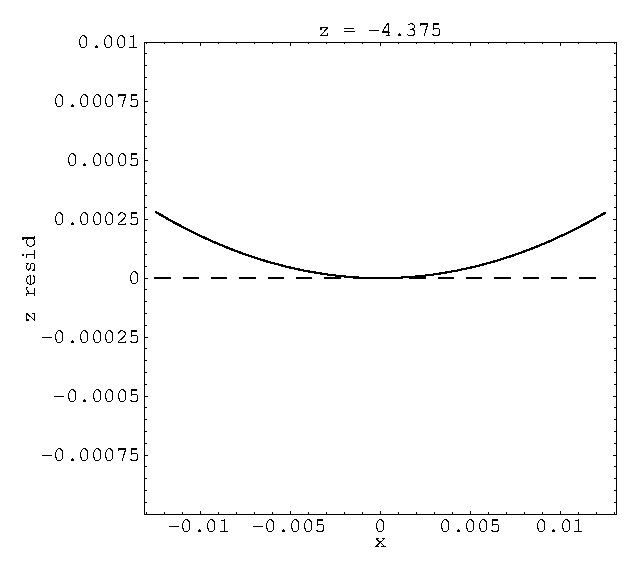
\includegraphics[width=7.3 cm]{layer1_right4.eps} &
    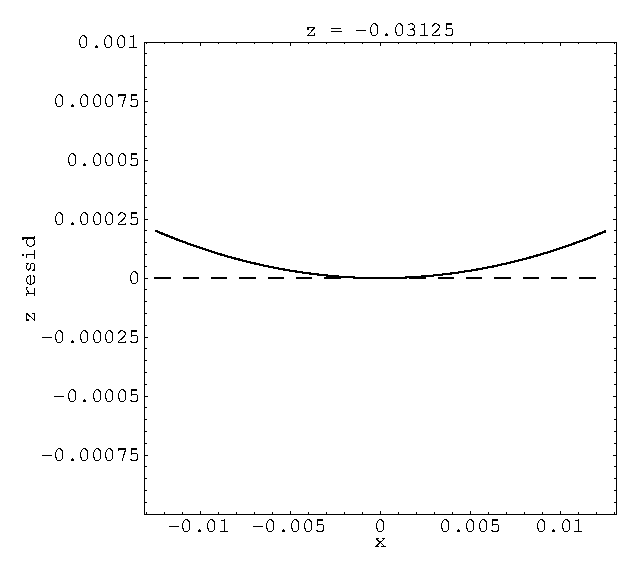
\includegraphics[width=7.3 cm]{layer1_right3.eps} \\
    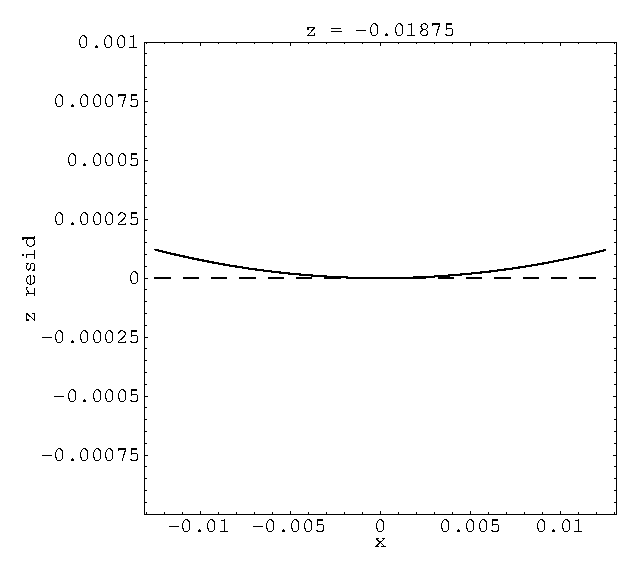
\includegraphics[width=7.3 cm]{layer1_right2.eps} &
    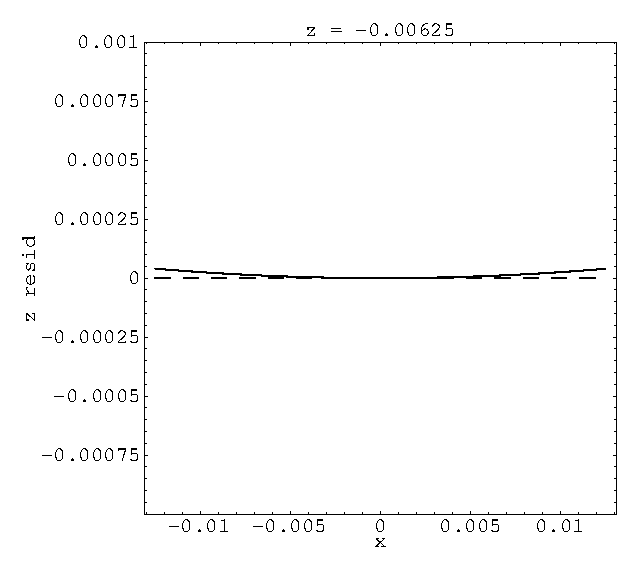
\includegraphics[width=7.3 cm]{layer1_right1.eps} \\
  \end{tabular}

\pagebreak

\subsection*{Layer 1 (Positive Z)}
  \begin{tabular}{c c}
    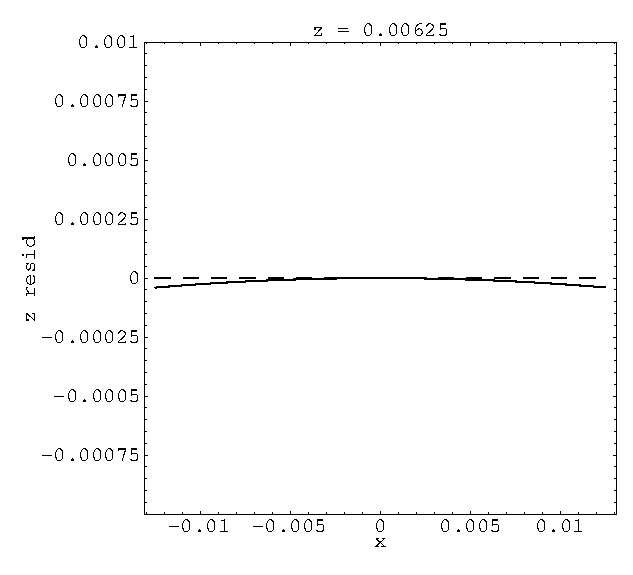
\includegraphics[width=7.3 cm]{layer1_left1.eps} &
    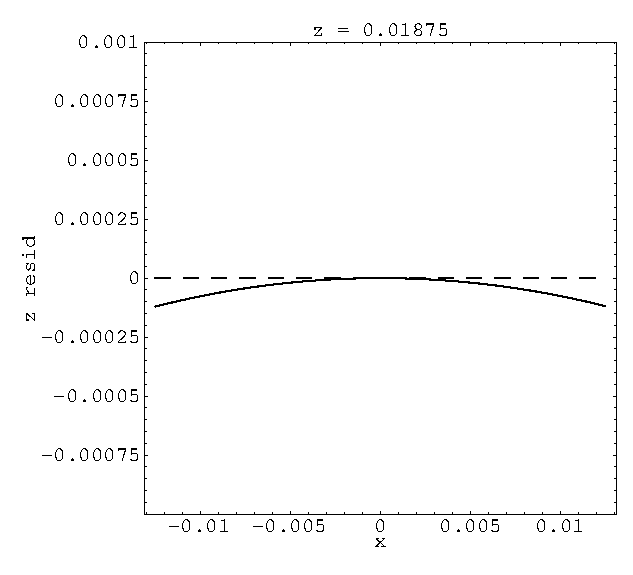
\includegraphics[width=7.3 cm]{layer1_left2.eps} \\
    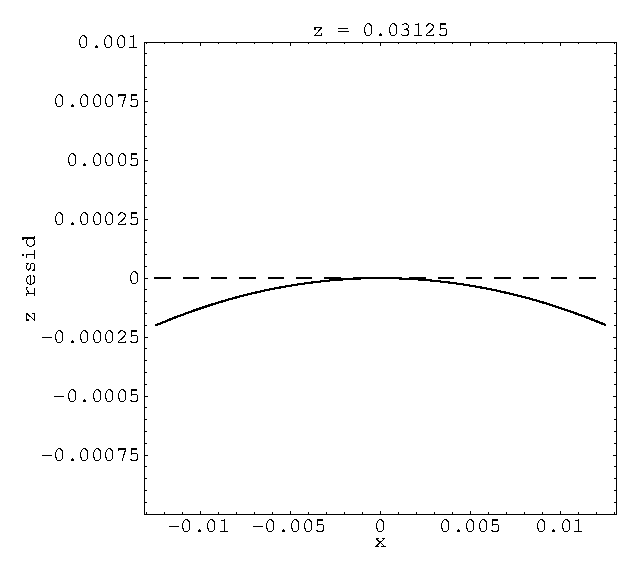
\includegraphics[width=7.3 cm]{layer1_left3.eps} &
    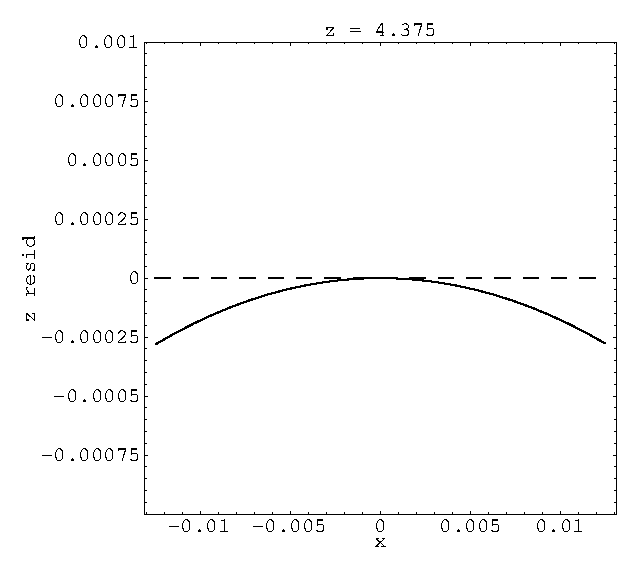
\includegraphics[width=7.3 cm]{layer1_left4.eps} \\
  \end{tabular}

\pagebreak

\subsection*{Layer 2}
  \begin{tabular}{c c}
    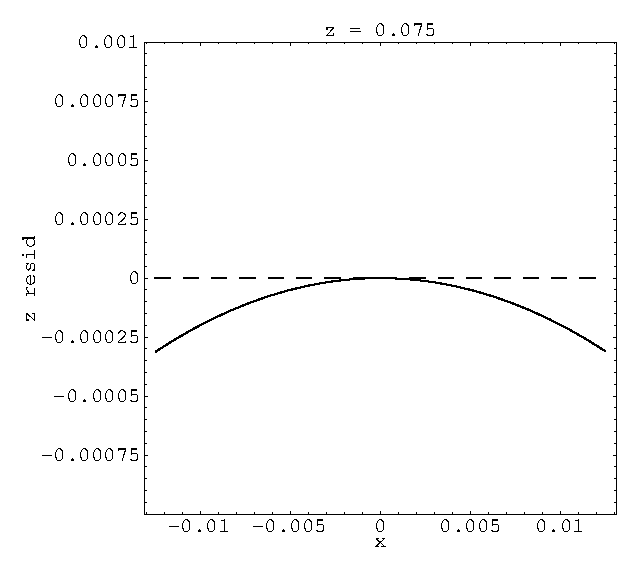
\includegraphics[width=7.3 cm]{layer2_left2.eps} &
    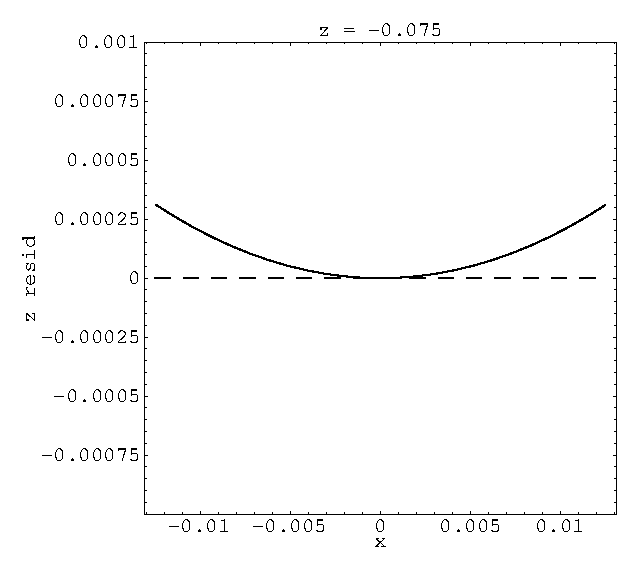
\includegraphics[width=7.3 cm]{layer2_right2.eps} \\
    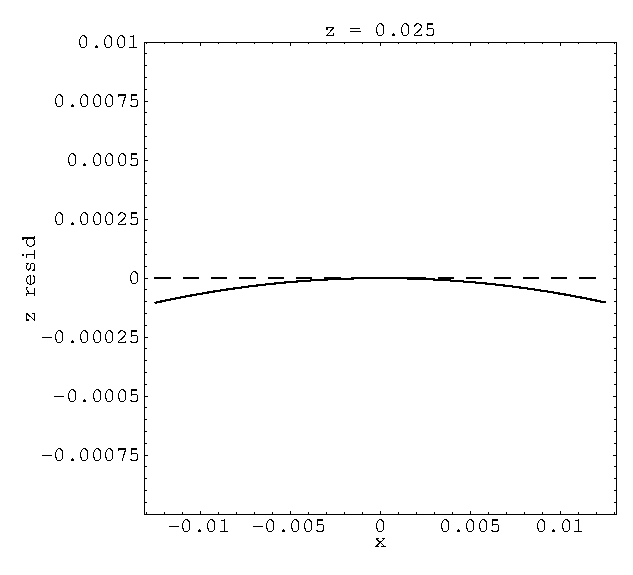
\includegraphics[width=7.3 cm]{layer2_left1.eps} &
    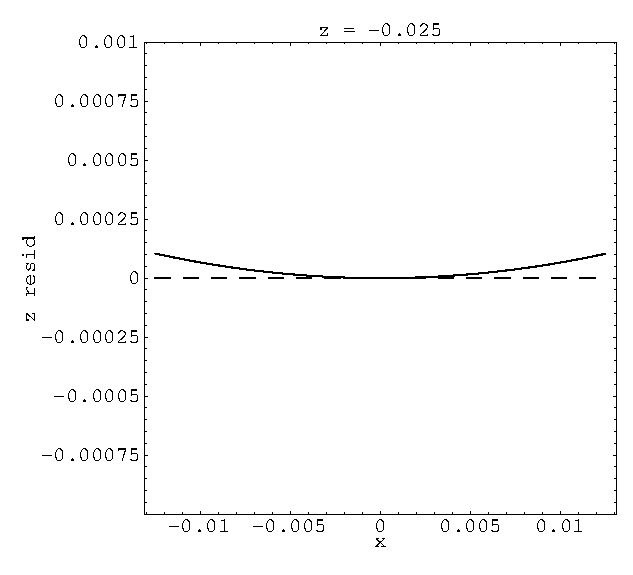
\includegraphics[width=7.3 cm]{layer2_right1.eps} \\
  \end{tabular}

\pagebreak

\subsection*{Layer 3}
  \begin{tabular}{c c}
    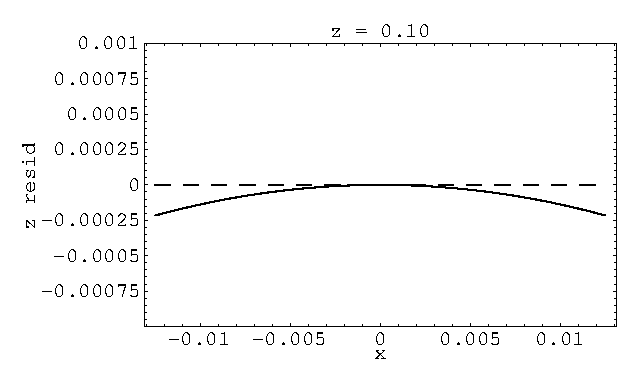
\includegraphics[width=7.3 cm]{layer3_left2.eps} &
    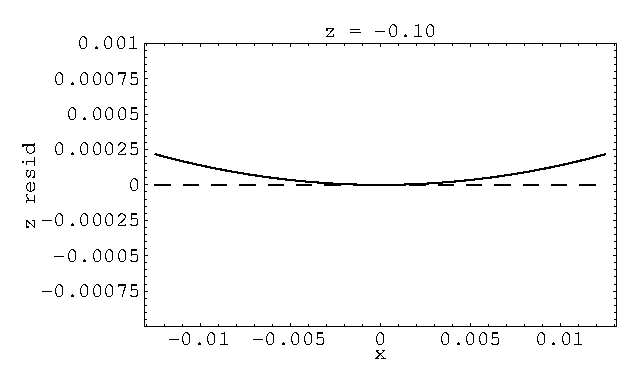
\includegraphics[width=7.3 cm]{layer3_right2.eps} \\
    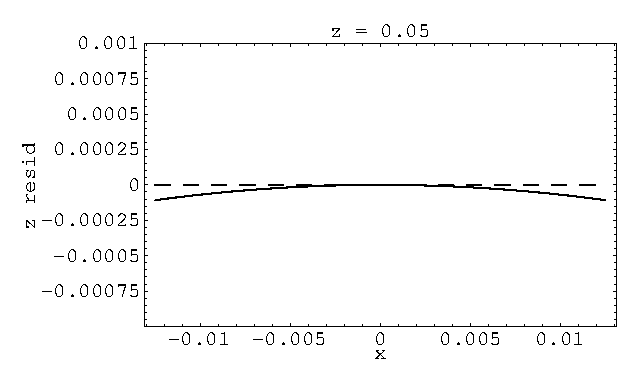
\includegraphics[width=7.3 cm]{layer3_left1.eps} &
    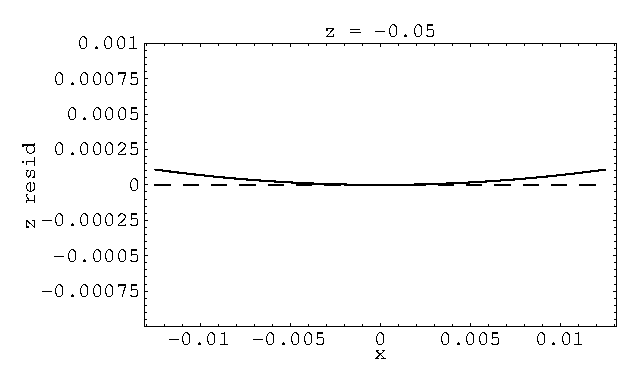
\includegraphics[width=7.3 cm]{layer3_right1.eps} \\
  \end{tabular}
  \begin{center}
    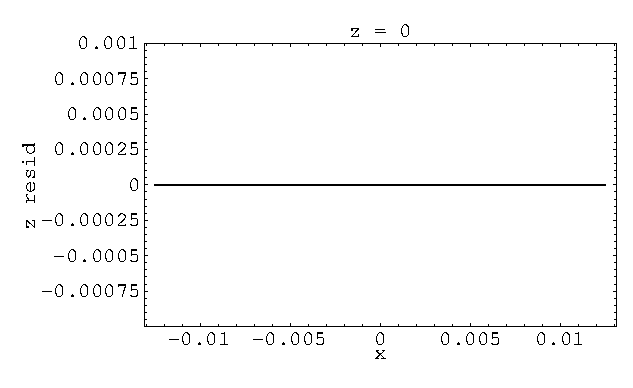
\includegraphics[width=7.3 cm]{layer3_middle.eps}
  \end{center}

\pagebreak

\subsection*{Layer 4}
  \begin{tabular}{c c}
    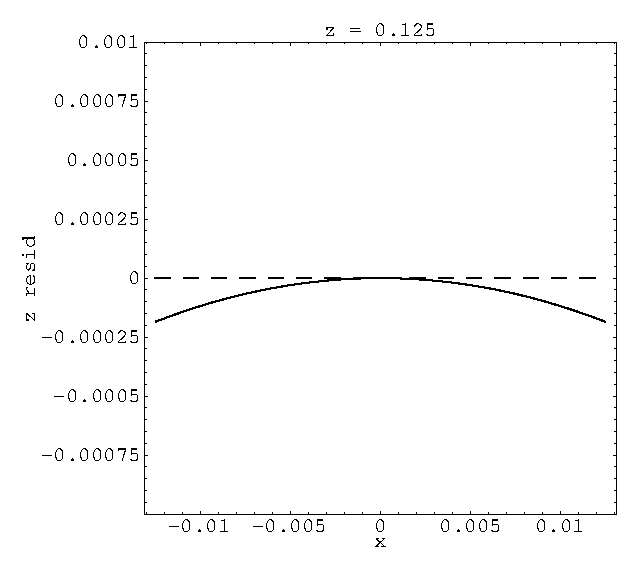
\includegraphics[width=7.3 cm]{layer4_left3.eps} &
    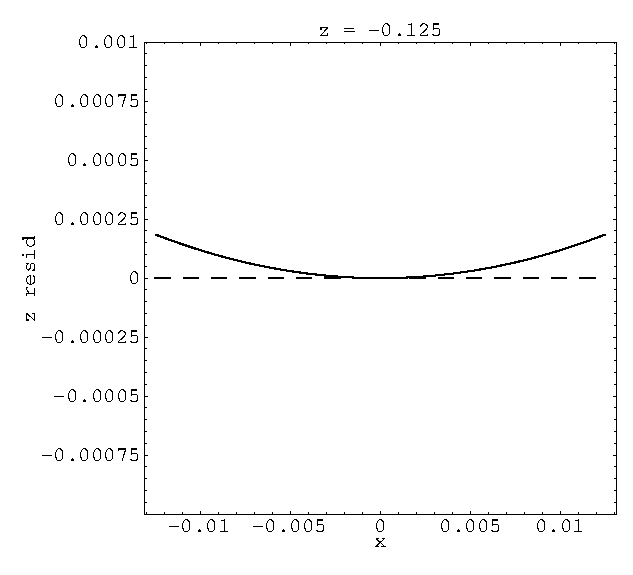
\includegraphics[width=7.3 cm]{layer4_right3.eps} \\
    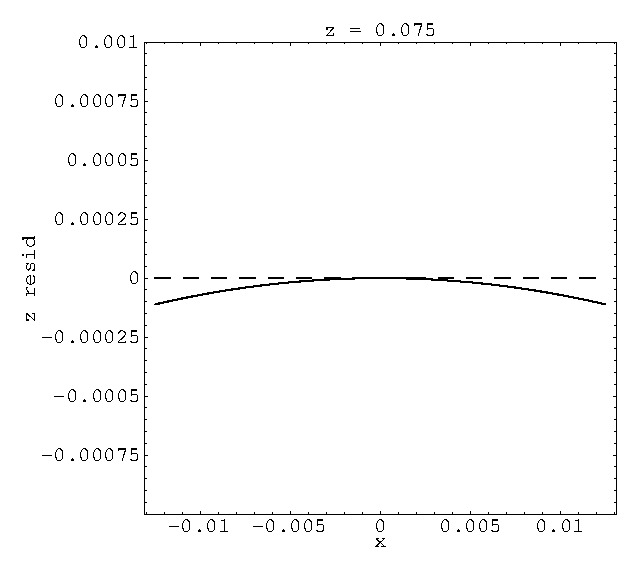
\includegraphics[width=7.3 cm]{layer4_left2.eps} &
    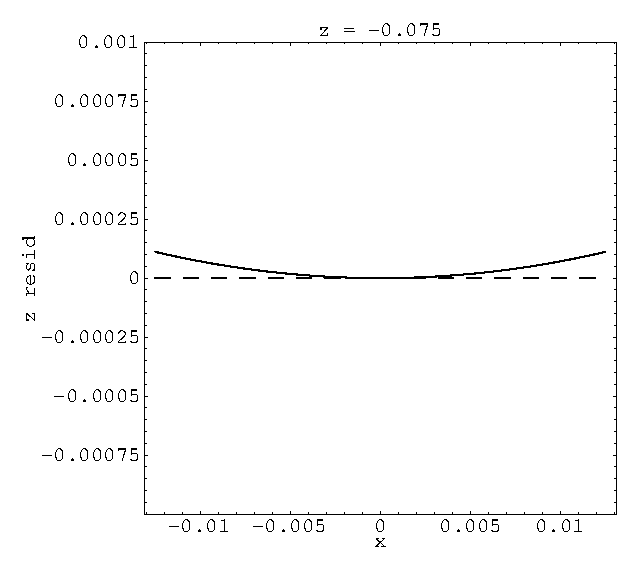
\includegraphics[width=7.3 cm]{layer4_right2.eps} \\
    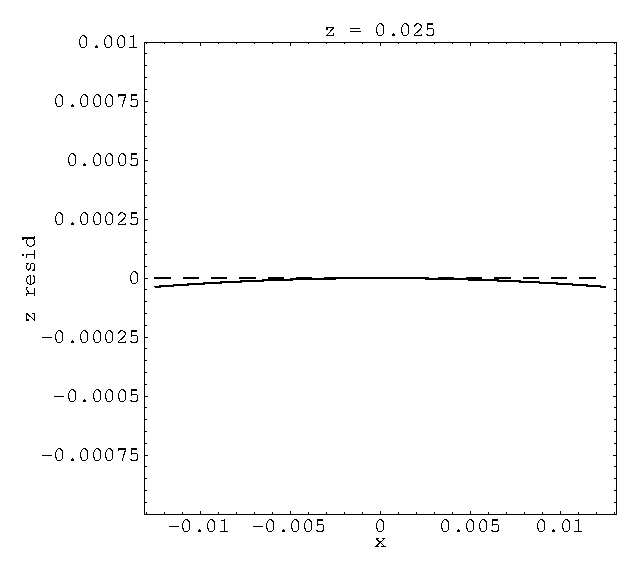
\includegraphics[width=7.3 cm]{layer4_left1.eps} &
    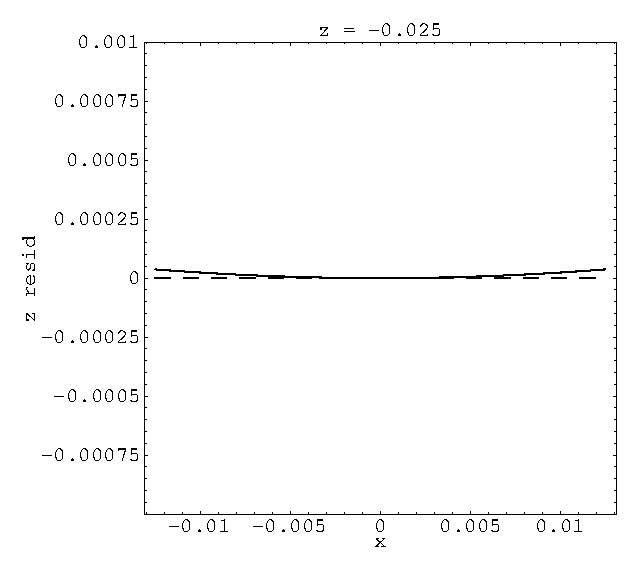
\includegraphics[width=7.3 cm]{layer4_right1.eps} \\
  \end{tabular}

\end{document}
